
\chapter{Manual de instalación y ejemplo de uso}
\section{Manual de instalación}
\subsection{Requisitos}
\begin{itemize}
    \item PHP 7.2
    \item Composer \cite{Composer}
    \item Apache
    \item MySQL o MariaDB    
\end{itemize}

\subsection{Pasos para la instalación}
\begin{enumerate}
    \item Descomprimir o copiar el repositorio en una carpeta
    \item Crear una nueva Base de datos en MySQL
    \item Copiar en el archivo ``app/config/dbMysqlCredentials.config.ph'' los datos de acceso \footnote{Se recomienda no usar el usuario root para acceder a la base de datos}
    \item Ejecutar desde MySQL los scripts de la carpeta sql en el orden que se indica: 
        \begin{enumerate}
            \item Database.ddl
            \item Views.sql
        \end{enumerate}
    \item En la carpeta ``app/dependencies'' ejecutar el siguiente comando
    composer install
    \item Apuntar hacia la carpeta app mediante un VirtualHost de Apache
    \item Acceder con el navegador en función de la ruta generada por Apache 
\end{enumerate}

\section{Ejemplo de uso} \label{capturas}
\subsection{Index}
En la imagen \ref{fig:index} se puede ver la página inicial de la aplicación. 
En ella los usuarios pueden copiar y pegar el correo para que sea analizado, además deben indicar al sistema qué tipo de mensaje es (EML, HTML o texto).
\begin{figure}[htb]
    \centering
    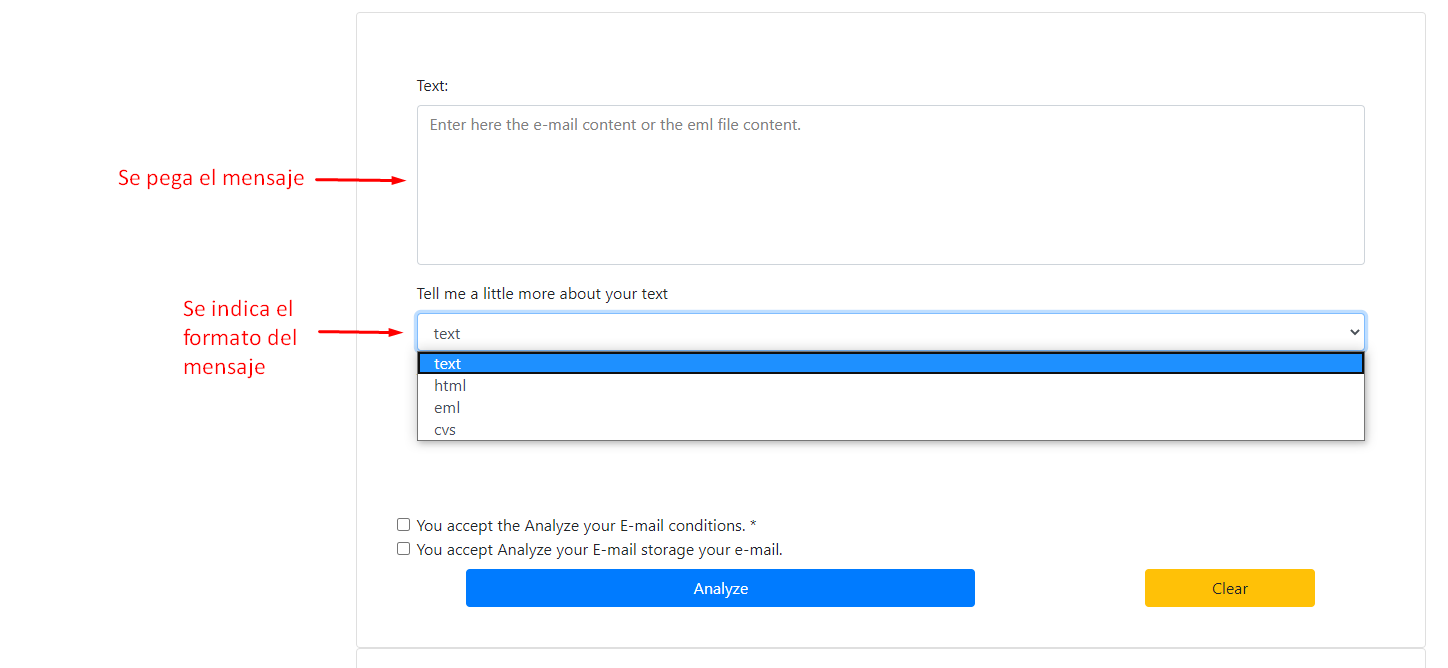
\includegraphics[width=\textwidth]{imagenes/capturasAplicacion/Analizar_mensaje.png}
\caption{Index de la aplicación}
\label{fig:index}
\end{figure}

\subsection{Mensaje}
Cuando un mensaje es analizado, el usuario verá algo parecido a las figuras \ref{fig:mensaje_datos} y \ref{fig:mensaje_patrones}. En la primera se puede ver la información básica del mensaje, como el formato, cuándo se añadió o cuándo se analizó. 

En la segunda figura \ref{fig:mensaje_patrones} se pueden ver qué patrones se han encontrado en dicho mensaje. Además, en caso de que el usuario quiera obtener más información sobre algún patrón en contro, simplemente podría clicar encima para ser redirigido a la página del patrón. 

\begin{figure}[htb]
    \centering
    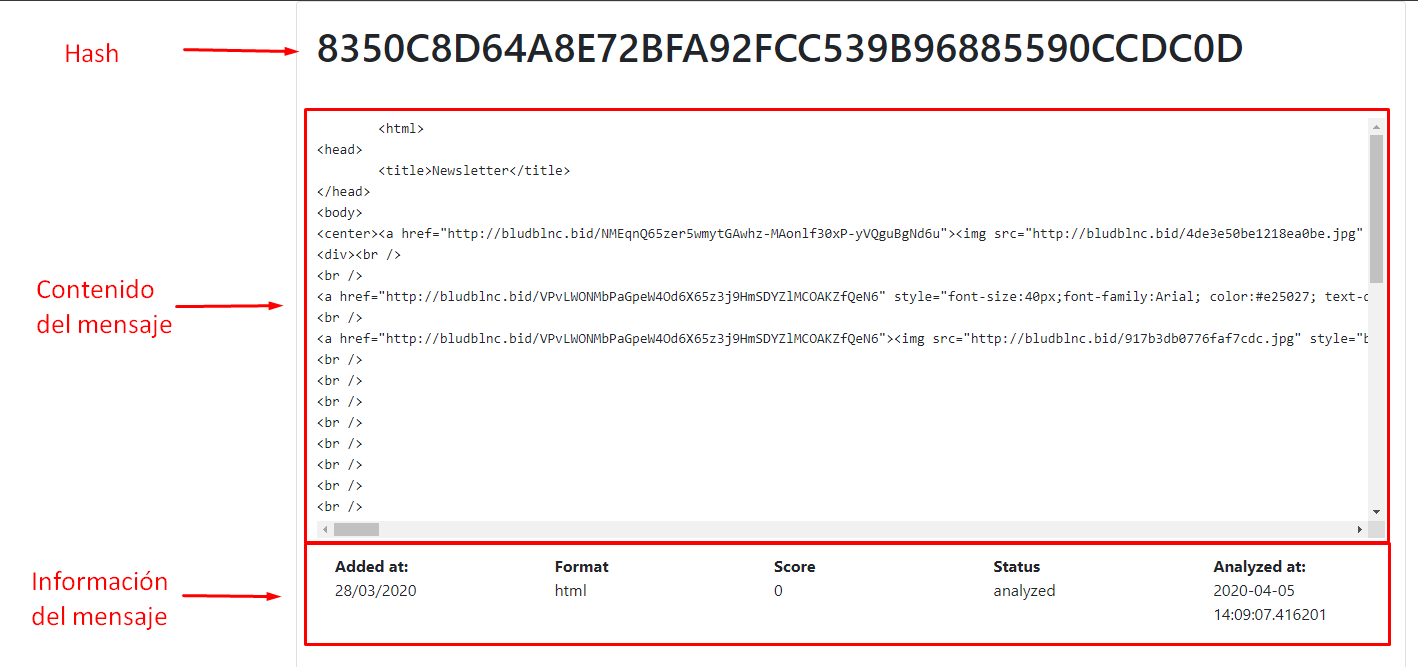
\includegraphics[width=0.8\textwidth]{imagenes/capturasAplicacion/Mensaje_info.png}
\caption{Vista de un mensaje: Información básica}
\label{fig:mensaje_datos}
\end{figure}

\begin{figure}[htb]
    \centering
    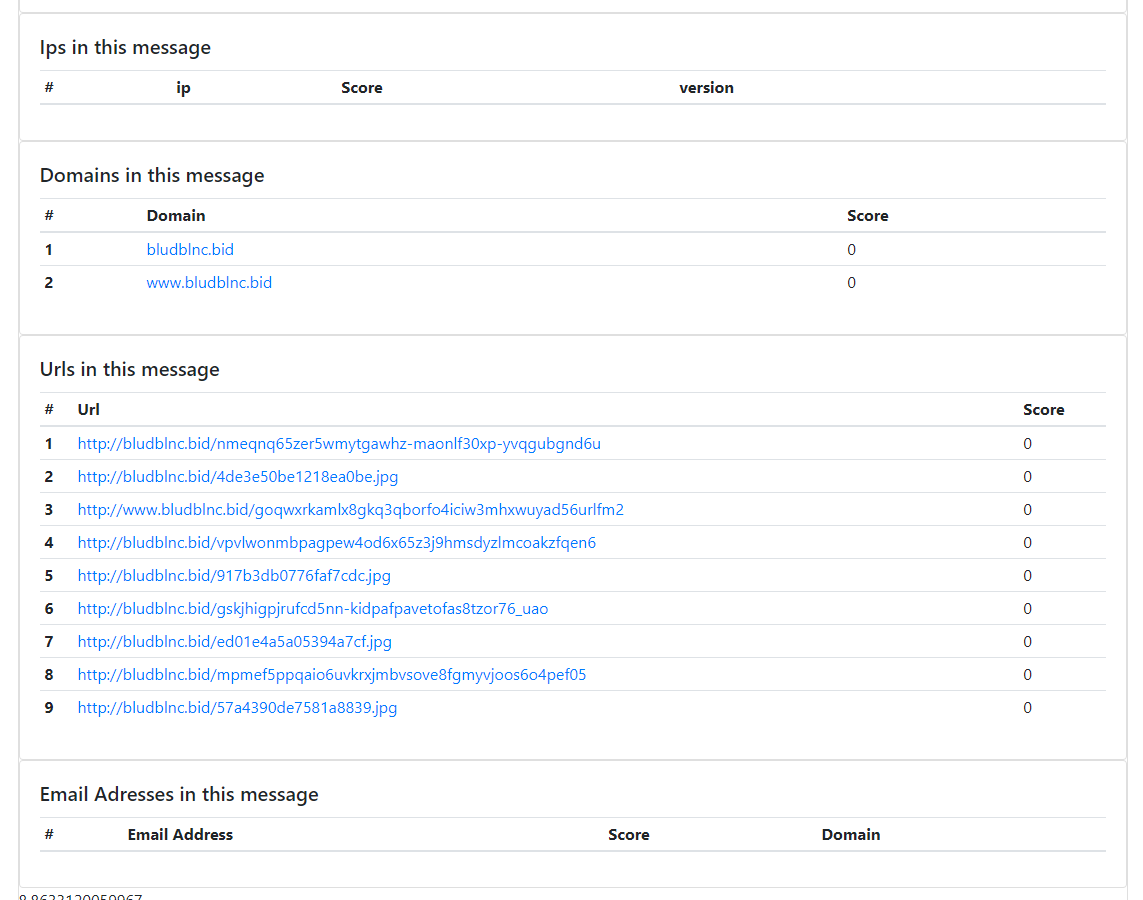
\includegraphics[width=0.8\textwidth]{imagenes/capturasAplicacion/Mensaje_patrones.png}
\caption{Vista de un mensaje: Patrones}
\label{fig:mensaje_patrones}
\end{figure}

\clearpage
\subsection{Dominio}
En el caso de los dominios, la información varía un poco dependiendo de si es un dominio (figura \ref{fig:dominio}) o un sundominio (figura \ref{fig:Subdominio}).

En caso de ser un subdominio, en la información básica aparecerá el dominio al que pertenece pudiendo navegar hacia él si se clica. 

Por otro lado, en caso de ser un dominio, aparecerán sus subdominios.

El resto de información como mensajes, enlaces, o direcciones de correo donde aparece este patrón, es idéntica y se puede navegar hacia ellos si se clica encima. 

\begin{figure}[htb]
    \centering
    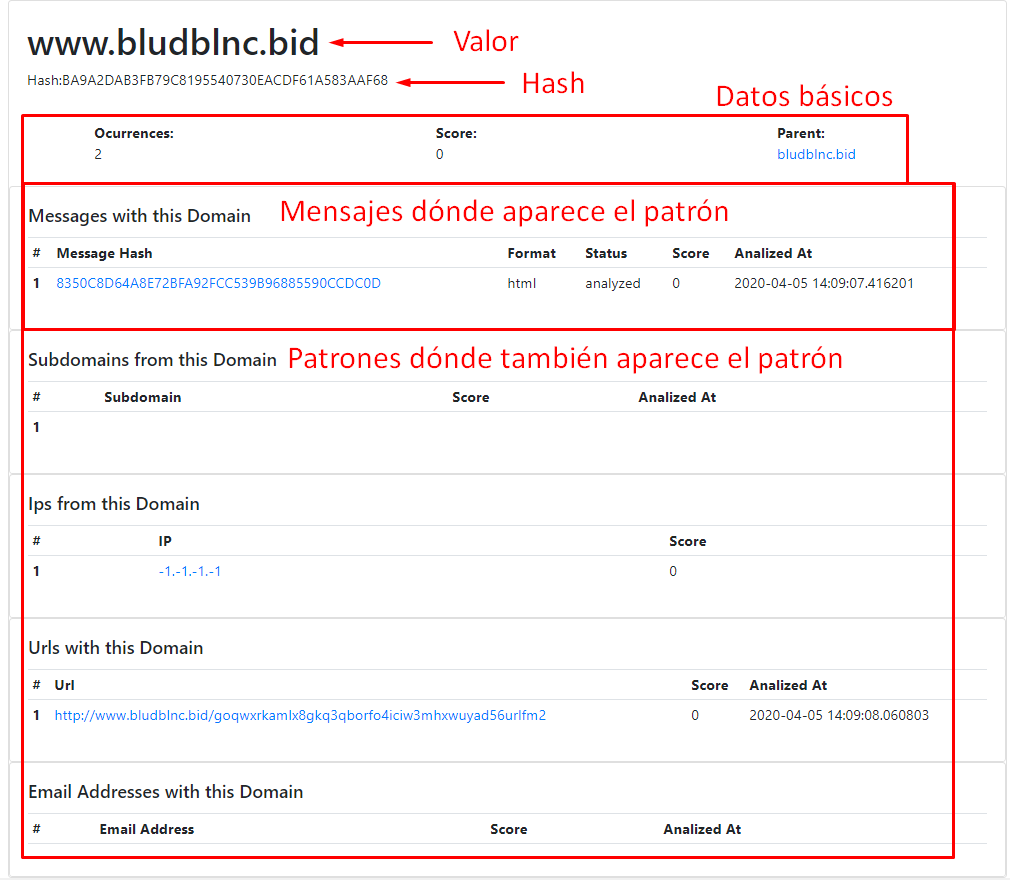
\includegraphics[width=0.9\textwidth]{imagenes/capturasAplicacion/Subdominio.png}
\caption{Vista de un subdominio.}
\label{fig:Subdominio}
\end{figure}


\begin{figure}[htb]
    \centering
    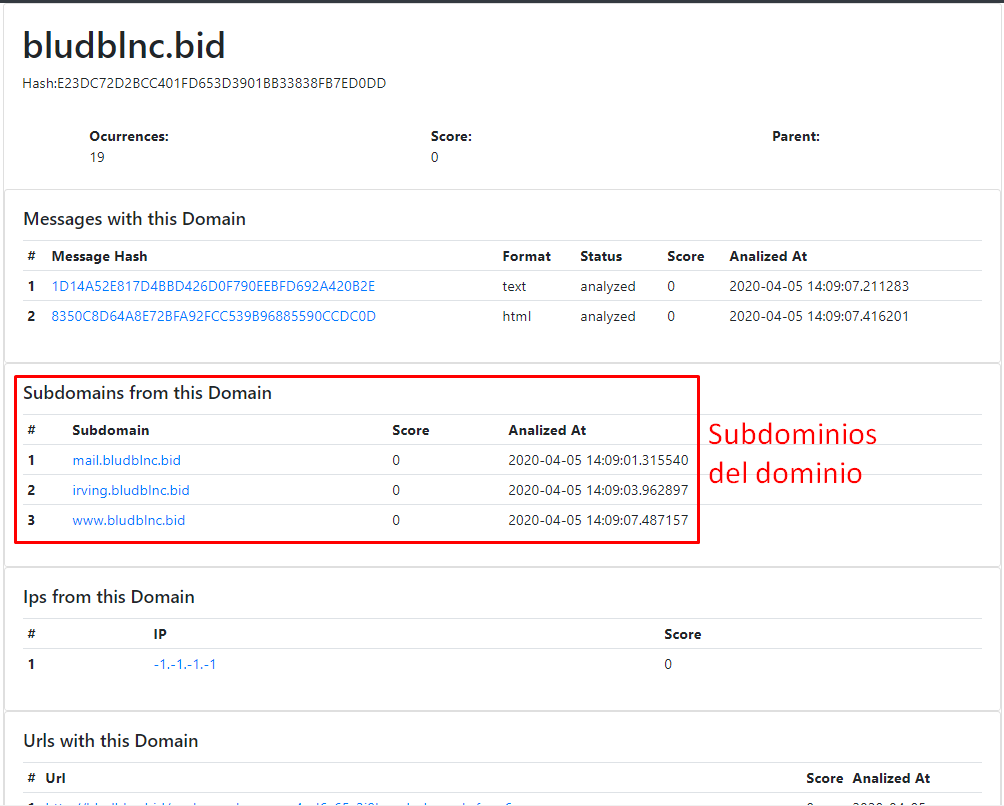
\includegraphics[width=0.9\textwidth]{imagenes/capturasAplicacion/Dominio.png}
\caption{Vista de un dominio.}
\label{fig:dominio}
\end{figure}

\clearpage
\subsection{Enlaces} \label{vista_enlaces}
En el caso de los enlaces, se ha integrado la plataforma con Virus Total, de modo que se puede analizar el enlace directamente desde la aplicación clicándo únicamente en el botón de \textit{Analyze} (Ver figuras \ref{fig:enlace} y \ref{fig:enlace_vt}).

\begin{figure}[htb]
    \centering
    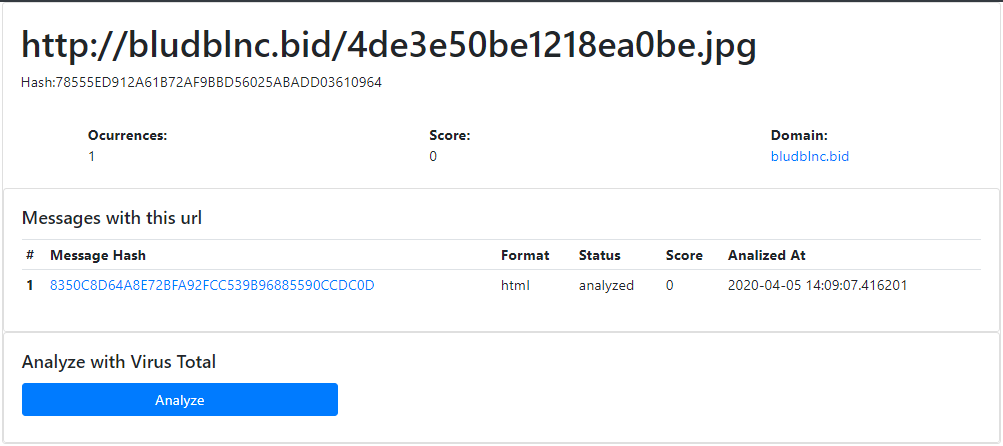
\includegraphics[width=0.8\textwidth]{imagenes/capturasAplicacion/Enlaces.png}
\caption{Vista de un enlace.}
\label{fig:enlace}
\end{figure}


\begin{figure}[htb]
    \centering
    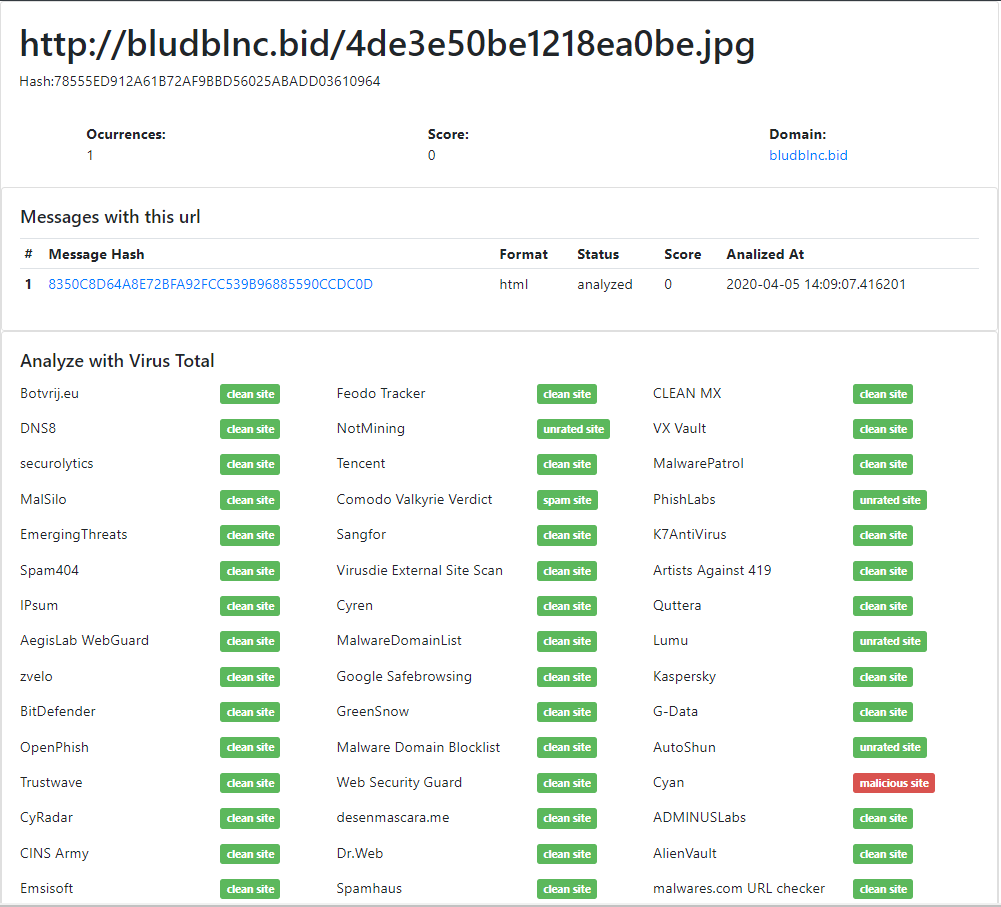
\includegraphics[width=0.8\textwidth]{imagenes/capturasAplicacion/Enlaces_virusTotal.png}
\caption{Vista de un enlace tras analizarlo con VirusTotal.}
\label{fig:enlace_vt}
\end{figure}

\clearpage
\subsection{Direcciones IP} \label{vista_ip}
Finalmente con las direcciones IP también se ha integrado el servicio de VirusTotal pudiendo analizar la dirección IP con este servicio (ver figuras \ref{fig:ip} y \ref{fig:ip_vt}).

\begin{figure}[htb]
    \centering
    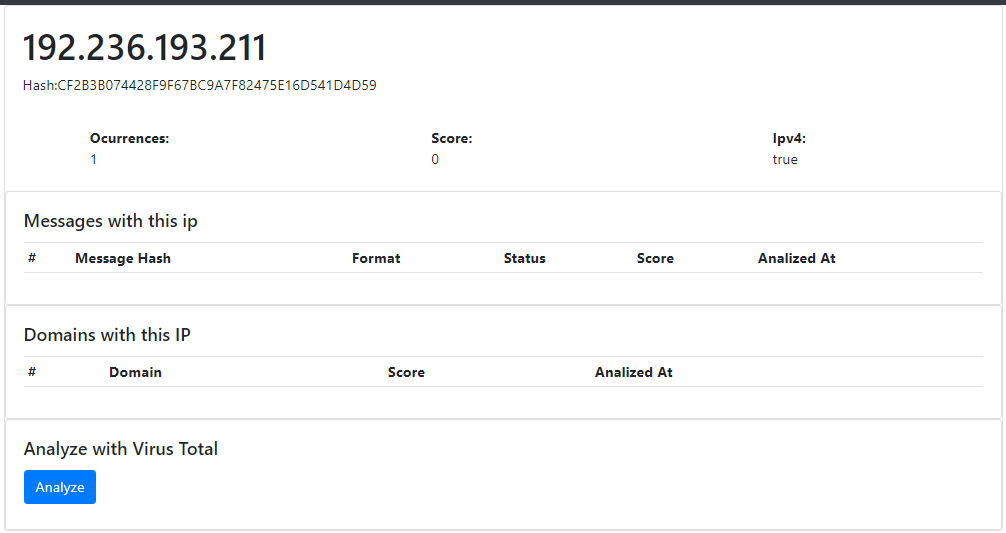
\includegraphics[width=0.8\textwidth]{imagenes/capturasAplicacion/IP.png}
\caption{Vista de una dirección IP.}
\label{fig:ip}
\end{figure}


\begin{figure}[htb]
    \centering
    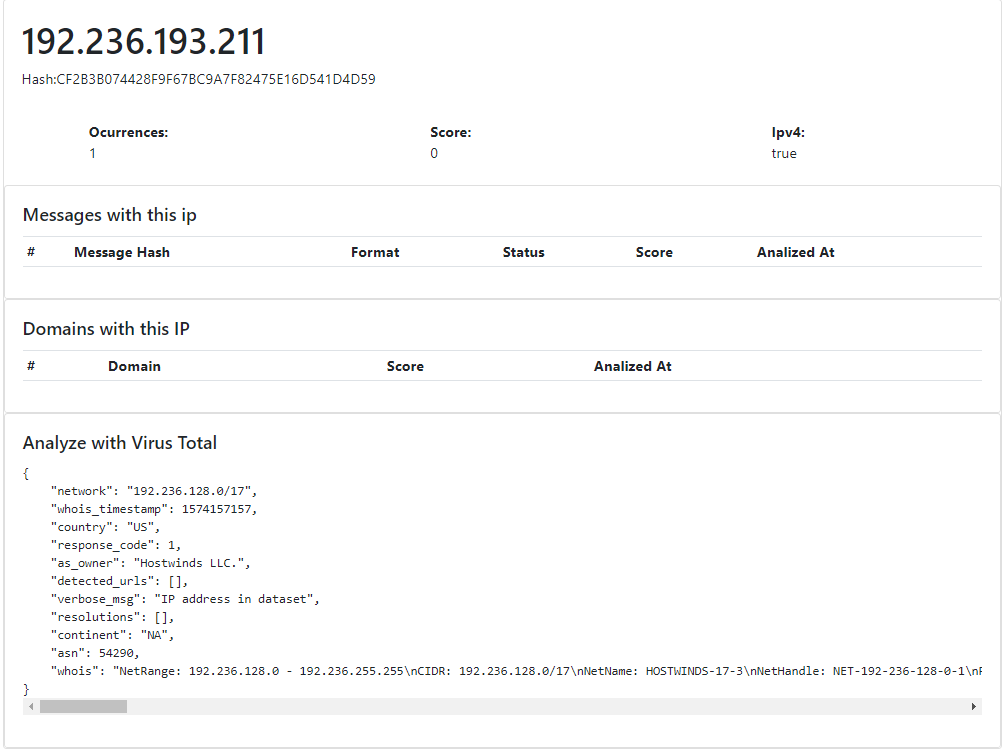
\includegraphics[width=0.8\textwidth]{imagenes/capturasAplicacion/IP_vt.png}
\caption{Vista de una dirección IP tras analizarla con VirusTotal.}
\label{fig:ip_vt}
\end{figure}